\documentclass{standalone}
\usepackage{tikz}
\usetikzlibrary{shapes.geometric}

\definecolor{lightblue}{RGB}{204,229,255}
\definecolor{lightpink}{RGB}{255,204,229}
\definecolor{lightorange}{RGB}{255,229,204}
\definecolor{blue}{RGB}{0,0,255}
\definecolor{magenta}{RGB}{255,0,128}

\tikzset{
  venn circle/.style={
    draw,
    ellipse,
    minimum width=4cm,
    minimum height=3cm,
    opacity=0.7,
    line width=1pt
  },
  title text/.style={
    font=\bfseries,
    align=center
  }
}

\begin{document}

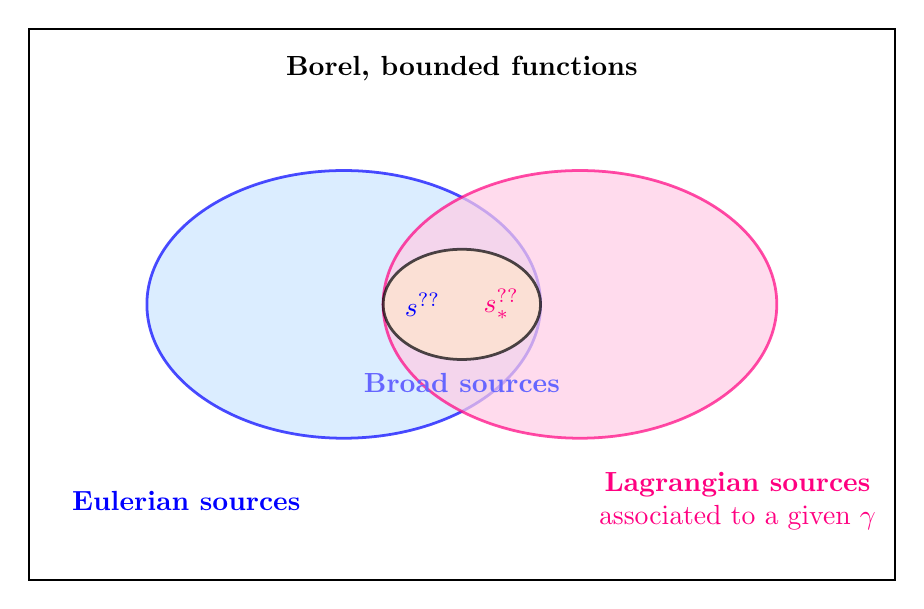
\begin{tikzpicture}
  % Draw the outer rectangle
  \draw[black, thick] (-5.5,-3.5) rectangle (5.5,3.5);
  
  % Title
  \node[title text] at (0,3) {Borel, bounded functions};
  
  % Draw the left ellipse (Eulerian sources)
  \filldraw[venn circle, draw=blue, fill=lightblue] (-1.5,0) ellipse (2.5cm and 1.7cm);
  
  % Draw the right ellipse (Lagrangian sources)
  \filldraw[venn circle, draw=magenta, fill=lightpink] (1.5,0) ellipse (2.5cm and 1.7cm);
  
  % Add the intersection fill (slightly darker)
  \filldraw[venn circle, fill=lightorange, opacity=0.7] (0,0) ellipse (1cm and 0.7cm);
  
  % Add labels
  \node[blue] at (-3.5,-2.5) {\textbf{Eulerian sources}};
  \node[magenta, align=center] at (3.5,-2.5) {\textbf{Lagrangian sources}\\associated to a given $\gamma$};
  
  % Add the text in the intersection
  \node[blue] at (-0.5,0) {$s^{??}$};
  \node[magenta] at (0.5,0) {$s_*^{??}$};
  \node[blue!60] at (0,-1) {\textbf{Broad sources}};
\end{tikzpicture}

\end{document}